\section*{Problem 2 Statement}

xxx

\section*{Solution}

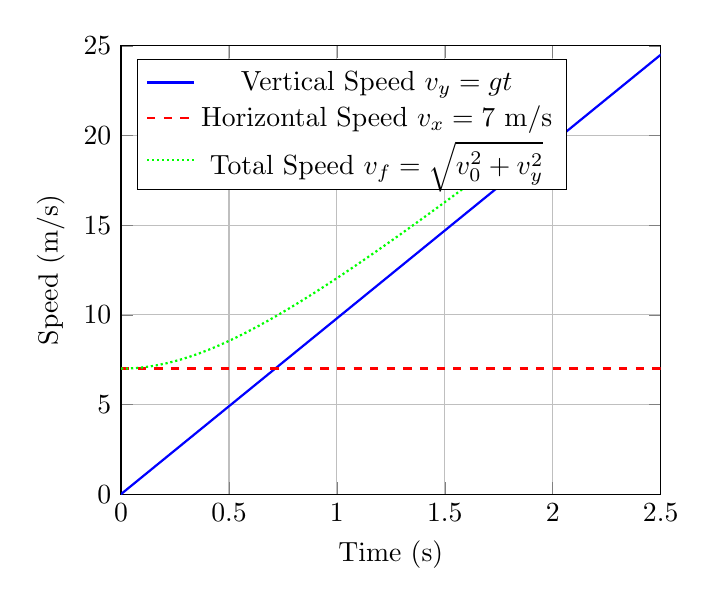
\begin{tikzpicture}
    \begin{axis}[
        xlabel={Time (s)},
        ylabel={Speed (m/s)},
        xmin=0, xmax=2.5,
        ymin=0, ymax=25,
        grid=major,
        legend pos=north west,
        samples=100,
    ]
    % Plot the vertical speed due to gravity
    \addplot[blue, thick] {9.8*x};
    \addlegendentry{Vertical Speed $v_y = gt$}
    
    % Plot the horizontal speed (constant)
    \addplot[red, thick, dashed] {7};
    \addlegendentry{Horizontal Speed $v_x = 7$ m/s}
    
    % Plot the total speed (resultant)
    \addplot[green, thick, densely dotted, domain=0:2.02] {sqrt(49 + (9.8*x)^2)};
    \addlegendentry{Total Speed $v_f = \sqrt{v_0^2 + v_y^2}$}
    
    \end{axis}
\end{tikzpicture}

xxx

\vfill
\subsection*{ANSWER}
\begin{enumerate}
    \item 1
    \item 2
\end{enumerate}